
\FloatBarrier\begin{figure}[!h]
\centering
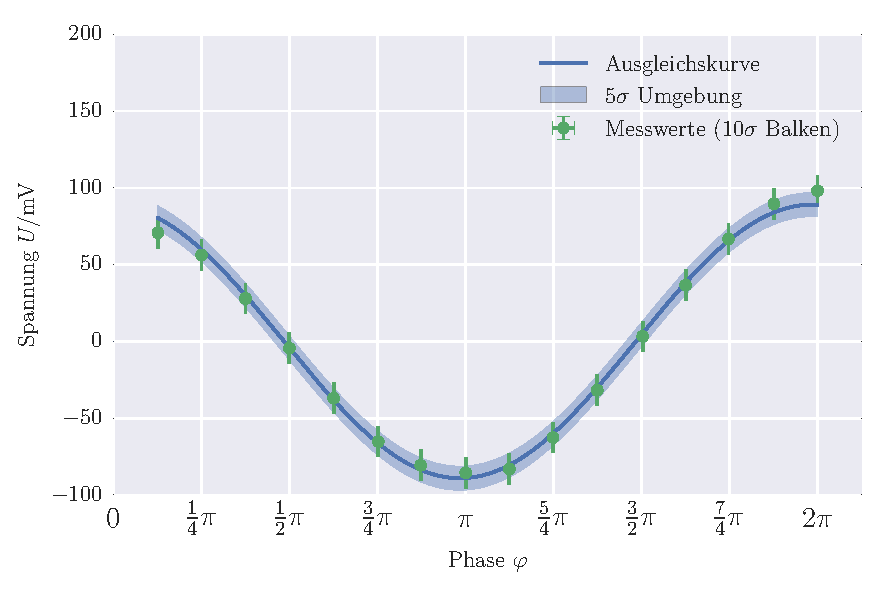
\includegraphics[scale=1]{../Grafiken/Phasenempfindlicher_Gleichrichter.pdf}
\caption{Darstellung der Abhängigkeit der Ausgangs-Gleichspannung des 
	Ringmodulators von der Phase $\varphi$ der Eingangs-Wechselspannungen. 
	Die Fehler der Messwerte sind aufgrund ihres geringen Wertes verzehnfacht
	dargestellt. Und auch das Fehlerband der Ausgleichskurve wurde mit fünf skaliert,
	um sichtbar zu sein.
	\label{fig:phasenempfindlicher_gleichrichter}}
\end{figure}
\FloatBarrier